\documentclass[11pt,a4paper]{article}
\usepackage[margin=2.5cm]{geometry}
\usepackage{amsmath,amssymb,bm}
\usepackage{graphicx}
\usepackage{float}
\usepackage{listings}
\usepackage{xcolor}

\lstset{language=Python,basicstyle=\ttfamily\small,breaklines=true,frame=single}

% Anything you still have to write shows up in red so it can't be missed.
\newcommand{\todo}[1]{\textcolor{red}{[TODO: #1]}}

\title{Image Analysis: Assignment 4}
\author{Elina Rosato}
\date{\today}

\begin{document}

\begin{titlepage}
    \centering
    \vspace*{2cm}

    {\Large Lund University\par}

    \vspace{1.5cm}

    {\large Course code: FMAN20\par}
    {\large Course name: Image Analysis\par}

    \vspace{3cm}

    {\Huge\bfseries Assignment 4\par}

    \vspace{3cm}

    {\large\itshape Elina Rosato\par}

    \vspace{2cm}

    \begin{tabular}{rl}
        Program: & MSc Program in Machine Learning, Systems and Control \\[4pt]
        Lecturer: & K. Magnus J. Oskarsson
    \end{tabular}

    \vfill

    {\large \today\par}
\end{titlepage}

%==============================================================
\section{Color correction of images}
%==============================================================

\subsection{Method}

The image $\bm g$ has a color cast and the image $\bm f$ has the correct colors. The color change is a linear
transformation, so for each pixel $\bm g(i,j)=A\,\bm f(i,j)$, where $\bm f(i,j)$ and $\bm g(i,j)$ are RGB vectors
with 3 numbers and $A$ is an unknown $3\times3$ matrix. When $A$ is found we get an estimate of the
original image from $\hat{\bm f}=A^{-1}\bm g$. Since some values can end up outside $[0,1]$, I clip them to that range.

The matrix $A$ has $9$ unknowns. One pixel gives $3$ equations (red, green and blue), so we need $9/3=3$ pixels.
\textbf{The minimum is 3 corresponding pixels.} If the three colors of $\bm f$ are the columns of $F$ and the
three colors of $\bm g$ are the columns of $G$, then $G=AF$ and $A=GF^{-1}$. This needs $F$ to be invertible,
which is not true if the three colors are almost the same.

The equation $\bm g=A\bm f$ is not true for all pixels. The black squares are in \texttt{task1\_org.png}
(that is $\bm f$), not in \texttt{task1\_color.png} as the task text says. Inside a square $\bm f=(0,0,0)$
but $\bm g$ has a normal color. These pixels are $6.7\%$ of the image and the other $93.3\%$ I call the
uncorrupted pixels. If a bad pixel is picked we get a bad $A$, so I used RANSAC, which tries many random samples
and keeps the best one. I repeat $200$ times:
\begin{enumerate}
  \item Pick $3$ random pixels and calculate $A=GF^{-1}$ (samples where $F$ is almost not invertible are skipped).
  \item For every pixel, calculate the error $\|\bm g-A\bm f\|$. If it is smaller than a threshold $\tau$,
    the pixel is an inlier. Count the inliers.
\end{enumerate}
The $A$ with the most inliers is kept. Finally I calculate $A$ again with least squares on all of its inliers,
which is more exact than using only $3$ pixels since the pixel values are rounded and a bit noisy.

\subsection{Choice of threshold}

I tried four values of $\tau$ (pixel values are between $0$ and $1$):

\begin{center}
\begin{tabular}{ccc}
 $\tau$ & Inliers & PSNR on uncorrupted pixels \\ \hline
 0.02 & 14.2\% & 32.94 \\
 0.05 & 83.2\% & 33.34 \\
 0.10 & 93.7\% & 33.02 \\
 0.20 & 94.0\% & 33.02 \\
\end{tabular}
\end{center}

With $\tau=0.02$ and $\tau=0.05$ the inliers are fewer than the $93.3\%$ uncorrupted pixels, so good pixels
are thrown away because of the noise. With $\tau=0.1$ the inliers are $93.7\%$, close to the real fraction, and
$\tau=0.2$ gives almost the same result. I chose $\tau=0.1$ for this reason and not for the PSNR.

\subsection{Results}

The estimated matrix is
\begin{equation}
  A=\begin{pmatrix}
     0.974 & -0.107 &  0.171\\
     0.117 &  0.774 & -0.164\\
    -0.132 &  0.208 &  0.865
  \end{pmatrix},
\end{equation}
and $2\,857\,020$ of $3\,048\,192$ pixels ($93.7\%$) were inliers. The code is in \texttt{task1.py}.

\begin{figure}[htbp]
  \centering
  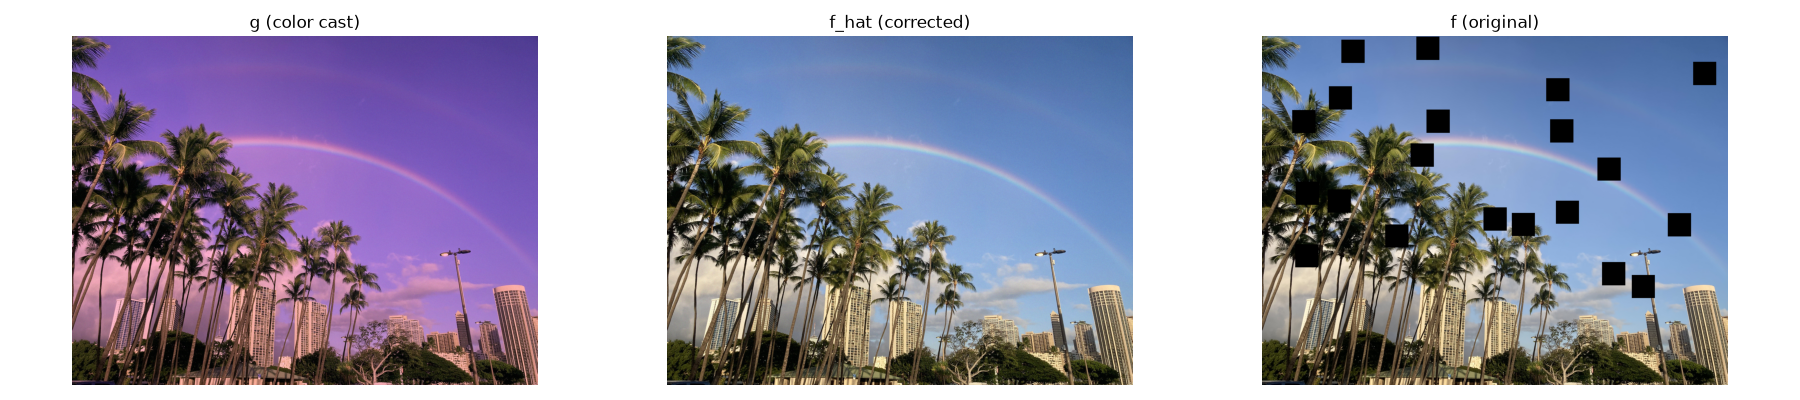
\includegraphics[width=\textwidth]{task1_comparison.png}
  \caption{Left: $\bm g$ with the color cast. Middle: my estimate $\hat{\bm f}=A^{-1}\bm g$ (saved as
  \texttt{task1\_corrected.png}). Right: the original $\bm f$ with the black squares.}
\end{figure}

The purple color is gone and $\hat{\bm f}$ looks like $\bm f$. In the black squares $\hat{\bm f}$ shows the real
image, since it is calculated from $\bm g$.

I compared $\hat{\bm f}$ with $\bm f$ using PSNR and SSIM (from \texttt{scikit-image}) and \reflectbox{F}LIP
(from \texttt{flip-evaluator}), and I did the same for $\bm g$ to see the improvement. PSNR is based on the
mean squared difference of the pixels, SSIM compares small windows (brightness, contrast, structure) and
\reflectbox{F}LIP measures how big the difference looks to a human. For SSIM and \reflectbox{F}LIP I took the mean of the
error map, either over the whole image or only over the uncorrupted pixels (a mask that is true where
$\bm f$ is not black).

\begin{center}
\begin{tabular}{llcc}
 & Metric & Whole image & Uncorrupted pixels \\ \hline
 $\hat{\bm f}$ vs.\ $\bm f$ & PSNR (dB, higher is better) & 16.37 & 33.02 \\
 & SSIM (higher is better) & 0.736 & 0.788 \\
 & \reflectbox{F}LIP (lower is better) & 0.118 & 0.070 \\ \hline
 $\bm g$ vs.\ $\bm f$ & PSNR (dB) & 15.43 & 19.70 \\
 & SSIM & 0.740 & 0.792 \\
 & \reflectbox{F}LIP & 0.537 & 0.464 \\
\end{tabular}
\end{center}

\subsection{Discussion}

On the whole image the PSNR only goes from $15.4$ to $16.4$\,dB, but on the uncorrupted pixels it goes from
$19.7$ to $33.0$\,dB. The reason is the black squares: there $\bm f$ is black and $\hat{\bm f}$ has the real
colors, so the error is large even though $A$ is not wrong. These pixels are only $6.7\%$ of the image but they
dominate the mean, so the numbers for the uncorrupted pixels show how good the color correction is.
\reflectbox{F}LIP agrees, the error goes from $0.464$ to $0.070$.

SSIM did not improve ($0.792$ for $\bm g$, $0.788$ for $\hat{\bm f}$). A possible reason is that SSIM looks at
structure like edges and textures and a color cast does not change this much, but I did not test it.

%==============================================================

\section{Segmentation with graph cuts}
%==============================================================

\subsection{Mean and standard deviation}

I assume that the intensities in each class follow a Gaussian distribution, and I estimated the mean $\mu$
and standard deviation $\sigma$ from the known values (2362 chamber values and 6854 background values):

\begin{center}
\begin{tabular}{lcc}
 & Mean $\mu$ & Standard deviation $\sigma$ \\ \hline
 Chamber & 0.3542 & 0.0992 \\
 Background & 0.1065 & 0.0936 \\
\end{tabular}
\end{center}

\subsection{Negative log likelihoods}

For a Gaussian, $P(f)=\frac{1}{\sqrt{2\pi}\sigma}e^{-(f-\mu)^2/(2\sigma^2)}$, so
\begin{equation}
  -\log P(f)=\log\!\big(\sqrt{2\pi}\,\sigma\big)+\frac{(f-\mu)^2}{2\sigma^2}.
\end{equation}
The first term comes from the normalizing constant and I leave it out, as the task says (it is almost the same for the
two classes since the $\sigma$ are almost equal). What is left is
\begin{equation}
  -\log P(f\,|\,\text{chamber})=\frac{(f-\mu_{\text{chamber}})^2}{2\sigma_{\text{chamber}}^2},\qquad
  -\log P(f\,|\,\text{background})=\frac{(f-\mu_{\text{background}})^2}{2\sigma_{\text{background}}^2}.
\end{equation}
These are small if the intensity is close to the mean of the class, so they work as the cost of giving a
pixel each label.

\subsection{The graph}

Every pixel is a node, and there is a source $s$ (the chamber side) and a sink $t$ (the background side).
The edges are:
\begin{itemize}
  \item between each pixel and its 4 neighbours, with weight $\nu$. If two neighbours get different labels an
    edge is cut, so these edges give $\nu$ times the length of the boundary;
  \item from the source to each pixel, with weight $-\log P(f\,|\,\text{background})$. It is cut if the
    pixel is on the sink side, i.e.\ if the pixel is called background;
  \item from each pixel to the sink, with weight $-\log P(f\,|\,\text{chamber})$. It is cut if the
    pixel is called chamber.
\end{itemize}
Every cut is a labeling of the image, and its cost is the energy (4) in the task, so the minimum cut gives the
best labeling. The minimum cut is found with the maximum flow from the source to the sink (\texttt{scipy}). The
pixels that can still be reached from the source after the max flow are the chamber pixels. The weights were
multiplied by $10000$ and rounded, since the max flow algorithm needs integers. The code is in \texttt{task2.py}.

\subsection{Choice of $\nu$ and result}

Figure~\ref{fig:nu} shows the result for several $\nu$. With $\nu=0$ every pixel just takes the cheaper
label, which gives many small spots. When $\nu$ grows the spots disappear and the boundary becomes smoother,
but with a large $\nu$ it becomes too stiff and cuts away parts of the chambers (see $\nu=8$). I chose $\nu=3$ as
a compromise.

\begin{figure}[H]
  \centering
  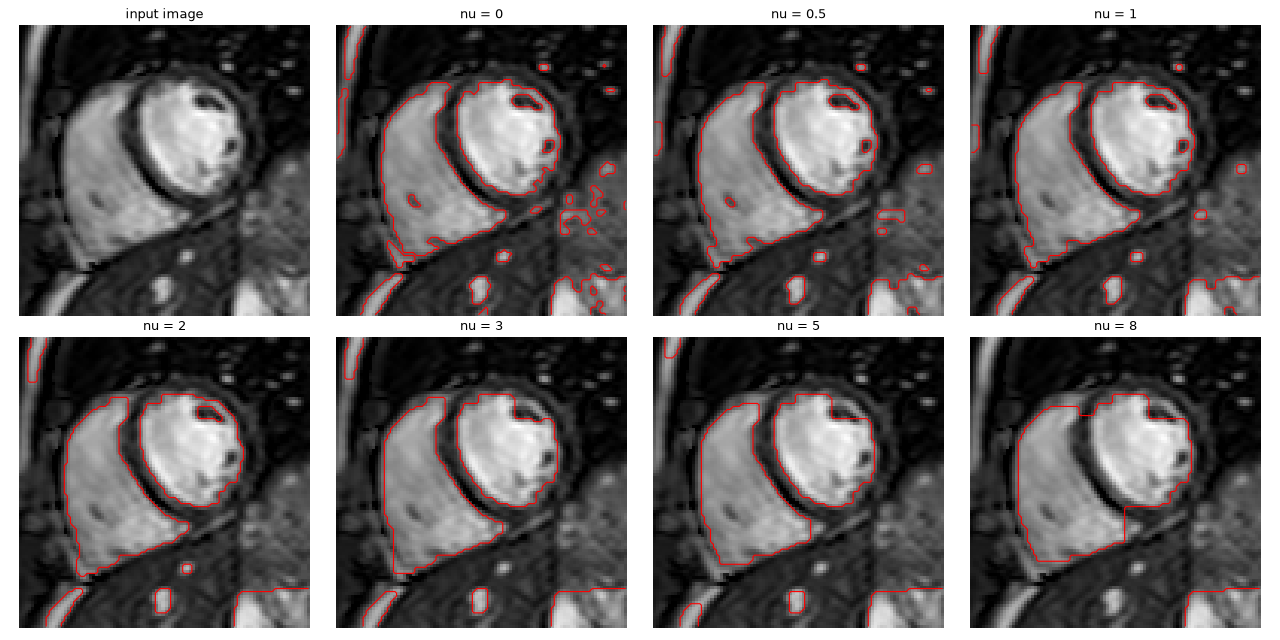
\includegraphics[width=0.7\textwidth]{task2_nu_comparison.png}
  \caption{The segmentation (red line) for different values of $\nu$.}\label{fig:nu}
\end{figure}

Figure~\ref{fig:heart} shows the input and the result for $\nu=3$.

\begin{figure}[H]
  \centering
  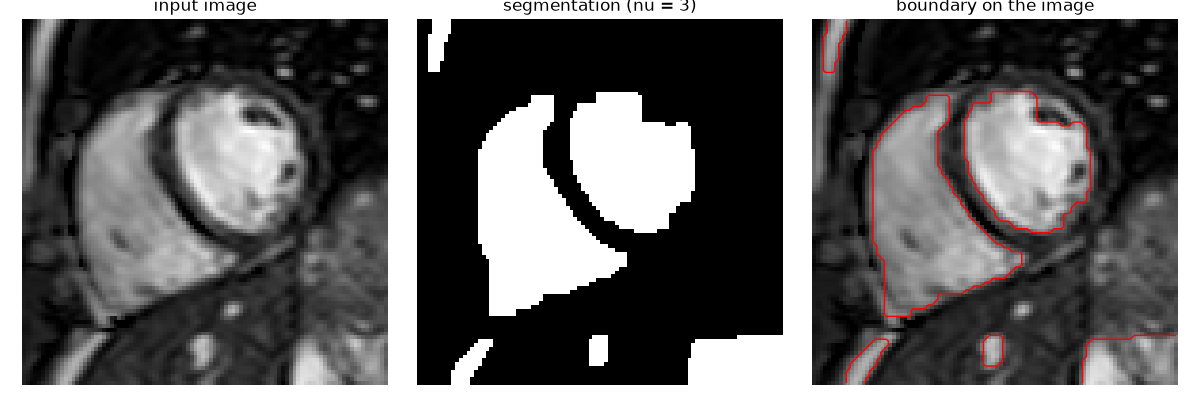
\includegraphics[width=0.7\textwidth]{task2_result.png}
  \caption{Left: the input image. Middle: the segmentation with $\nu=3$ (white is chamber).
  Right: the boundary on the image.}\label{fig:heart}
\end{figure}

Both chambers are found and the boundary
follows them well. The result is not perfect: other bright parts, for example the bottom right corner and a strip at the left
edge, are also labeled as chamber. Their intensities are like the chambers and the method only uses intensity
and boundary length, so it cannot tell the difference. I did not do the optional part 3.

%==============================================================
\section{Computer vision}
%==============================================================

A 3D point $U=(X,Y,Z)$ is projected to the image by writing it with an extra $1$, $(X,Y,Z,1)^T$, and
multiplying with the camera matrix $P_1$. This gives three numbers $(a,b,c)^T=P_1(X,Y,Z,1)^T$, and the image
point is $(a/c,\,b/c)$. A point can be the 3D point of the detected point $u=(6,-\tfrac12)$ only if
this gives exactly $u$. I calculate this for the three points, with
\begin{equation}
  P_1=\begin{pmatrix}1&2&3&3\\3&2&0&-2\\1&1&2&0\end{pmatrix}.
\end{equation}

\noindent$U_1=(2,\tfrac12,1)$:
\begin{equation}
  P_1\begin{pmatrix}2\\ \tfrac12\\1\\1\end{pmatrix}
  =\begin{pmatrix}2+1+3+3\\ 6+1+0-2\\ 2+\tfrac12+2+0\end{pmatrix}
  =\begin{pmatrix}9\\5\\ \tfrac92\end{pmatrix}
  \ \Rightarrow\ \Big(\frac{9}{9/2},\frac{5}{9/2}\Big)=\Big(2,\tfrac{10}{9}\Big)\neq u.
\end{equation}

\noindent$U_2=(\tfrac13,\tfrac13,0)$:
\begin{equation}
  P_1\begin{pmatrix}\tfrac13\\ \tfrac13\\0\\1\end{pmatrix}
  =\begin{pmatrix}\tfrac13+\tfrac23+0+3\\ 1+\tfrac23+0-2\\ \tfrac13+\tfrac13+0+0\end{pmatrix}
  =\begin{pmatrix}4\\-\tfrac13\\ \tfrac23\end{pmatrix}
  \ \Rightarrow\ \Big(\frac{4}{2/3},\frac{-1/3}{2/3}\Big)=\Big(6,-\tfrac12\Big)=u.
\end{equation}

\noindent$U_3=(-12,18,1)$:
\begin{equation}
  P_1\begin{pmatrix}-12\\18\\1\\1\end{pmatrix}
  =\begin{pmatrix}-12+36+3+3\\ -36+36+0-2\\ -12+18+2+0\end{pmatrix}
  =\begin{pmatrix}30\\-2\\8\end{pmatrix}
  \ \Rightarrow\ \Big(\frac{30}{8},\frac{-2}{8}\Big)=\Big(\tfrac{15}{4},-\tfrac14\Big)\neq u.
\end{equation}

\textbf{Answer:} only $U_2=(\tfrac13,\tfrac13,0)$ can project to the detected point $u$. It is the only
one of the three points that gives exactly $(6,-\tfrac12)$ after the division by the third coordinate.

%==============================================================
\section{The garment classification system, part 4}
%==============================================================

\subsection{Version 1}

Version 1 is the system from Assignment 3. \texttt{im2segment} thresholds the image at 20 and finds the connected
components, \texttt{segment2feature} gives 10 shape numbers (for example the aspect ratio and the number of
holes), and \texttt{feature2class} is a $k$-nearest-neighbour classifier trained on the 1000 training segments
(it chose $k=1$). I ran the benchmark script on the five datasets. The hitrates (the fraction of the garments that
were classified correctly) were:

\begin{center}
\begin{tabular}{lcc}
 Dataset & Version 1 & Version 2 \\ \hline
 short1 & 60.0\% & 82.0\% \\
 short2 & 30.0\% & 74.0\% \\
 home1  & 48.9\% & 79.4\% \\
 home2  & 50.1\% & 77.6\% \\
 home3  & 44.3\% & 77.8\% \\
\end{tabular}
\end{center}

Version 1 did not go well. Only short1 ($60.0\%$) and home2 ($50.1\%$) are
above $50\%$, and short2 is only $30.0\%$. To find out why, I measured the two main steps separately.
The benchmark pairs the $i$-th segment with the $i$-th ground-truth garment, so the segmentation must find exactly
the right garments in the right order. The table shows the mean Jaccard index of the segmentation, in how many images
the number of segments was right (``Right no.''), and the hitrate if the classifier gets the ground-truth segments (``True segm.''):

\begin{center}
\small
\begin{tabular}{lccc|ccc}
 & \multicolumn{3}{c|}{Version 1} & \multicolumn{3}{c}{Version 2} \\
 Dataset & Jaccard & Right no. & True segm. & Jaccard & Right no. & True segm. \\ \hline
 short1 & 0.945 & 100\% & 80.0\% & 0.946 & 100\% & 78.0\% \\
 short2 & 0.775 & 70\%  & 68.0\% & 0.941 & 100\% & 74.0\% \\
 home1  & 0.896 & 87\%  & 68.7\% & 0.955 & 100\% & 78.8\% \\
 home2  & 0.894 & 88\%  & 71.9\% & 0.955 & 100\% & 80.6\% \\
 home3  & 0.862 & 82.5\% & 66.1\% & 0.956 & 100\% & 78.1\% \\
\end{tabular}
\end{center}

For version 1 there are two problems. First, the segmentation: a fixed threshold of 20 does not work for dark garments
or dim parts of a garment, which are broken into pieces or lose parts (short2 has many dark garments, and there the
right number of segments was found in only $70\%$ of the images). One extra or missing segment moves all later garments one position,
so all of them become wrong, which is why short2 is so bad (Figure~\ref{fig:thr} shows an example). This costs $20$ to $38$ percentage points (compare the hitrate
with the hitrate on the true segments). Second, the classifier: even with perfect segments it only
reaches $66$--$80\%$. The 10 hand-made features are on very different scales, which is not good for a distance based
method, and the classes are similar (a pullover, a coat and a shirt have almost the same silhouette).

\begin{figure}[H]
  \centering
  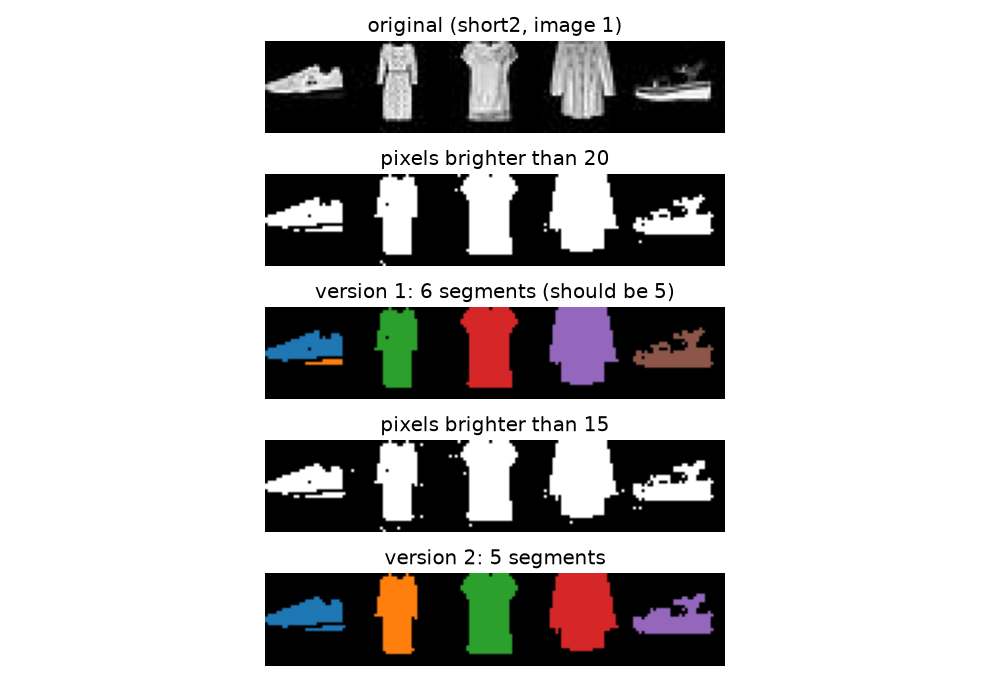
\includegraphics[width=0.8\textwidth]{threshold_example.png}
  \caption{An image from short2. Rows from top to bottom: the original; the pixels brighter than 20; the segments of
  version 1 (one color per segment); the pixels brighter than 15; the segments of version 2. The sole of the shoe is darker than 20, so
  version 1 makes it a separate segment and finds 6 segments instead of 5. Version 2 keeps the shoe in one piece.}\label{fig:thr}
\end{figure}

\subsection{Version 2}

I changed all three steps.

\begin{itemize}
  \item \textbf{Segmentation.} I lowered the threshold to 15, removed tiny specks and filled holes in the garments, so that
    dark garments stay in one piece. Then I use that every image has 5 garments in a row: I look at which columns of the image
    contain garment pixels, and cut the image at the 4 widest empty gaps. This always gives exactly 5 segments in the right
    (left to right) order. If there are too few gaps (garments that touch) the code uses connected components instead, but
    this was never needed on the five datasets. The threshold is not sensitive: values from 10 to 20 gave similar Jaccard indices.
  \item \textbf{Features.} Instead of the 10 numbers I use the silhouette of the garment: cut out the bounding box, put it in the middle
    of a square (so the shape is not stretched) and scale it to $20\times20$ pixels, plus the aspect ratio. This gives 401 numbers and does not depend
    on the size of the garment, which matters since the garments in the home datasets are up to $70$ pixels high but the training garments are $28$.
  \item \textbf{Classifier.} I use a support vector machine with an RBF kernel, after standardizing every feature. I tested other
    classifiers (k-nearest-neighbour, logistic regression, random forest, LDA) with 5-fold cross-validation on the 1000 training segments, and the
    SVM was among the best ($80.6\%$ against $74.2\%$ for version 1 with the old features). I set $C=10$ in the same way. I did not tune the classifier on the five datasets.
\end{itemize}

The results are in the table above. Version 2 reaches $74$ to $82\%$ on all five datasets, so the aim of more than $50\%$ is reached
everywhere. The segmentation now finds 5 segments in every image and the Jaccard index is about $0.95$ on all datasets. The difference
between the hitrate on the true segments and on my own segments is now at most about $3$ percentage points (on short1 it is even $4$ points higher, which is just
chance with 50 garments), so the segmentation does not cost much any more. The classifier also became better, from $66$--$80\%$ to $74$--$81\%$ with perfect segments, and this
is now what limits the system.

\subsection{Remaining errors and limitations}

Over all $3100$ garments in the five datasets, version 2 got $78.3\%$ right (version 1 got $47.7\%$). Most of the errors are between garments that
have similar silhouettes: pullover and coat are mixed up, and shirts are often classified as coat, pullover or T-shirt (only $39\%$ of
the shirts are correct, against $92\%$ for trousers and $95\%$ for ankle boots). The system only sees the shape of the segment, not the
texture or the colors, so these classes are hard to separate. A way to improve this would be to give the classifier information from the gray values
of the garment, but the benchmark only gives the segment to \texttt{segment2feature}, so I did not do it.

The segmentation uses that there are always exactly 5 garments in a row, which is true for these datasets but would not hold for other
layouts. The datasets with only 10 images (short1 and short2) have 50 garments each, so their hitrates are uncertain by about $\pm6$ percentage
points. I chose the threshold 15 after looking at the Jaccard index on these datasets, but since the result is almost the same from 10 to 20 I do not
think this matters.

\end{document}
